% !TeX program = xetex
\documentclass[xcolor={table,usenames,dvipsnames}]{beamer}
\usepackage{eso-pic} 
\usepackage[absolute,overlay]{textpos}
\usepackage{colortbl}
\usepackage{fourier}
\usepackage{booktabs}% http://ctan.org/pkg/booktabs
\newcommand{\tabitem}{~~\llap{\textbullet}~~}
\usepackage{tabularx}
\setbeamertemplate{blocks}[rounded][shadow=true]
\let\olditem\item
\renewcommand{\item}{%
\olditem\vspace{0pt}}     
\usepackage{ragged2e}


%\usepackage[round]{natbib} % incompatible avec biblatex
\usepackage{hyperref}
\hypersetup{
    colorlinks=true,
    linkcolor=.,
    filecolor=deepblue,      
    urlcolor=deepblue,
    pdftitle={Overleaf Example},
    pdfpagemode=FullScreen,
    citecolor=deepblue
    }
\definecolor{LightCyan}{rgb}{0.88,1,1}   
\usepackage[justification=centering]{caption}
\captionsetup{font=scriptsize}
\captionsetup[figure]{name=Fig.}
\captionsetup[table]{name=Tab.}
\setbeamertemplate{caption}[numbered]
\usepackage[T1]{fontenc}
\usepackage{ctex}
\UseRawInputEncoding
%\usepackage[backend=bibtex, style=authoryear, natbib=true, sorting=nty, backref=true]{biblatex}
\usepackage[style=authoryear, maxbibnames=99, mincitenames=1, maxcitenames=2, backref=true, hyperref=true, dashed=false, firstinits=true, backend=bibtex, bibencoding=utf8, uniquename=false, uniquelist=false, natbib=true]{biblatex}
\renewcommand*{\bibfont}{\footnotesize}
\setbeamerfont{footnote}{size=\tiny}

% Remove quotation marks from titles
\DeclareFieldFormat[article,incollection,inproceedings,conference]{title}{#1} 
\addbibresource{bibliographie.bib}

%\usepackage[backend=bibtex,
%style=authoryear,
%natbib=true,
%sorting=nty,
%backref=true
%]{biblatex}

\let\oldnocite\nocite
\makeatletter
\renewcommand*{\nocite}[1]{\oldnocite{#1}\Hy@backout{#1}}
\makeatother

\renewcommand*{\bibfont}{\footnotesize}

\DeclareCiteCommand{\cite}
  {\usebibmacro{prenote}}
  {\usebibmacro{citeindex}%
   \printtext[bibhyperref]{\usebibmacro{cite}}}
  {\multicitedelim}
  {\usebibmacro{postnote}}

\DeclareCiteCommand*{\cite}
  {\usebibmacro{prenote}}
  {\usebibmacro{citeindex}%
   \printtext[bibhyperref]{\usebibmacro{citeyear}}}
  {\multicitedelim}
  {\usebibmacro{postnote}}

\DeclareCiteCommand{\parencite}[\mkbibparens]
  {\usebibmacro{prenote}}
  {\usebibmacro{citeindex}%
    \printtext[bibhyperref]{\usebibmacro{cite}}}
  {\multicitedelim}
  {\usebibmacro{postnote}}

\DeclareCiteCommand*{\parencite}[\mkbibparens]
  {\usebibmacro{prenote}}
  {\usebibmacro{citeindex}%
    \printtext[bibhyperref]{\usebibmacro{citeyear}}}
  {\multicitedelim}
  {\usebibmacro{postnote}}

\DeclareCiteCommand{\footcite}[\mkbibfootnote]
  {\usebibmacro{prenote}}
  {\usebibmacro{citeindex}%
  \printtext[bibhyperref]{ \usebibmacro{cite}}}
  {\multicitedelim}
  {\usebibmacro{postnote}}

\DeclareCiteCommand{\footcitetext}[\mkbibfootnotetext]
  {\usebibmacro{prenote}}
  {\usebibmacro{citeindex}%
   \printtext[bibhyperref]{\usebibmacro{cite}}}
  {\multicitedelim}
  {\usebibmacro{postnote}}

%\DeclareCiteCommand{\textcite}
%  {\boolfalse{cbx:parens}}
%  {\usebibmacro{citeindex}%
%   \printtext[bibhyperref]{\usebibmacro{textcite}}}
%  {\ifbool{cbx:parens}
%     {\bibcloseparen\global\boolfalse{cbx:parens}}
%     {}%
%   \multicitedelim}
%  {\usebibmacro{textcite:postnote}}

        \DeclareCiteCommand{\textcite}
        {\usebibmacro{cite:init}%
            \usebibmacro{prenote}}
        {\usebibmacro{citeindex}%
            \printtext[bibhyperref]{\usebibmacro{textcite}}}
        {}
        {\printtext[bibhyperref]{\usebibmacro{textcite:postnote}}%
            \usebibmacro{cite:post}}

%\addbibresource{bibliographie.bib}

% Cannot enable in Xelatex
\usepackage{pgfpages}
% \setbeameroption{hide notes} % Only slides
% \setbeameroption{show only notes} % Only notes
% \setbeameroption{show notes on second screen}

% other packages
\usepackage{latexsym,amsmath,multicol,booktabs,calligra}
\usepackage{graphicx,listings,stackengine}
\usepackage[greek,french]{babel}
\usepackage[LGR,T1]{fontenc}
\usepackage{fontspec}

%\usepackage[sfdefault,light,led=.85]{merriweather} %% Option 'black' gives heavier bold face 


\usepackage[sfdefault]{AlegreyaSans} %% Option 'black' gives heavier bold face
%% The 'sfdefault' option to make the base font sans serif
\renewcommand*\oldstylenums[1]{{\AlegreyaSansOsF #1}}



% Define a command for text in Greek. Replace 'Gentium Plus' with a font of your choice if necessary.
%\newfontfamily\greekfont{Gentium Plus}
%\newcommand{\textgreek}[1]{{\greekfont #1}}

\DefineBibliographyStrings{french}{%
  backrefpage = {voir p\adddot},%
  backrefpages = {voir pp\adddot}%
}
\DeclareFieldFormat{pagerefformat}{\mkbibparens{{\color{red}\mkbibemph{#1}}}}
\renewbibmacro*{pageref}{%
  \iflistundef{pageref}
    {}
    {\printtext[pagerefformat]{%
       \ifnumgreater{\value{pageref}}{1}
         {\bibstring{backrefpages}\ppspace}
         {\bibstring{backrefpage}\ppspace}%
       \printlist[pageref][-\value{listtotal}]{pageref}}}}
\usepackage{wasysym}
% Enable only in Xelatex
 \usepackage{pstricks}

\author[Ljudmila PETKOVIC]{\small \textbf{Ljudmila PETKOVIC}\textsuperscript{1,2,3,4}\\\medskip{\footnotesize\texttt{prenom.nom@sorbonne-universite.fr}}}
\title[]{\fontsize{13pt}{13pt}\selectfont bbb}
%\subtitle{Approche \textit{PatternRank}}
\institute [JE \og{}Humanités numériques\fg{}] {\tiny \textsuperscript{1} Sorbonne Université, Faculté des Lettres, \textsc{UFR} Littératures françaises et comparée, \textsc{ED III} (\textsc{ED019})\\\textsuperscript{2} Sorbonne Université, Centre d'étude de la langue et des littératures françaises (\textsc{CELLF}), \textsc{UMR 8599}\\\textsuperscript{3} Sorbonne Université, Observatoire des textes, des idées et des corpus (\textsc{ObTIC})\\\textsuperscript{4} Sorbonne Université, \textsc{UFR} Sociologie et Informatique pour les Sciences Humaines}
\date[Séminaire doctoral \textsc{ObTIC}, 13/03/2025]{\scriptsize Séminaire doctoral \textsc{ObTIC} \\\textsc{SCAI}, salle du Conseil\\Paris, le \today}
\usepackage{YTU}

% defs
\def\cmd#1{\texttt{\color{red}\footnotesize $\backslash$#1}}
\def\env#1{\texttt{\color{blue}\footnotesize #1}}
\definecolor{deepblue}{rgb}{0,0,0.5}
\definecolor{deepred}{rgb}{0.6,0,0}
\definecolor{deepgreen}{rgb}{0,0.5,0}
\definecolor{halfgray}{gray}{0.55}
\definecolor{warmblack}{rgb}{0.0, 0.26, 0.26}
\newcommand{\bolder}[1]{{\color{purple}\bfseries#1}}
\lstset{
    basicstyle=\ttfamily\small,
    keywordstyle=\bfseries\color{deepblue},
    emphstyle=\ttfamily\color{deepred},    % Custom highlighting style
    stringstyle=\color{deepgreen},
    numbers=left,
    numberstyle=\small\color{halfgray},
    rulesepcolor=\color{red!20!green!20!blue!20},
    frame=shadowbox,
}
% \logo{%
%     
\includegraphics[width=1cm,height=1cm,keepaspectratio]{pic/obtic.jpg}~%
%     
\includegraphics[width=1cm,height=1cm,keepaspectratio]{pic/Lettres_su_logo.png}~%
% }
\usepackage{enumerate}
%\setbeamertemplate{section in toc}{\hspace*{1em}\inserttocsectionnumber.~\inserttocsection\par}
\setbeamertemplate{subsection in toc}{\hspace*{2em}\inserttocsectionnumber.\inserttocsubsectionnumber.~\inserttocsubsection\par}
\renewcommand*{\bibfont}{\scriptsize}



\let\oldfootnotesize\footnotesize
\renewcommand*{\footnotesize}{\oldfootnotesize\scriptsize}

%\setbeamertemplate{itemize/enumerate body begin}{\small}
\setbeamertemplate{itemize/enumerate subbody begin}{\small}
%
%\newcommand{\leftquote}{{\fontfamily{lmr}\selectfont\textquotedblleft}}
%\newcommand{\rightquote}{{\fontfamily{lmr}\selectfont\textquotedblright}}
%\newcommand{\leftguillemet}{{\fontfamily{lmr}\selectfont\guillemotleft}}
%\newcommand{\rightguillemet}{{\fontfamily{lmr}\selectfont\guillemotright}}


\setbeamertemplate{itemize subitem}{\textcolor{blue}{$\circ$}}




\begin{document}

\begin{frame}
    \titlepage
\begin{figure}
    \centering
    
    
\includegraphics[width=2cm,height=1cm,keepaspectratio]{pic/Lettres_su_logo.png}~\hspace*{0.5cm}%\includegraphics{}
    
\includegraphics[width=2cm,height=1cm,keepaspectratio]{pic/cellf.png}~\hspace*{0.5cm}%
    
\includegraphics[width=3cm,height=1cm,keepaspectratio]{pic/obtic.jpg}~%

\end{figure}
    
    \begin{note}
        {Introduce your self}
    \end{note}

\end{frame}

\section[Contributions de Charcot]{Contributions principales de Charcot}

\begin{frame}{Termes inventés par Charcot : référence}
	\begin{tabular}{rl}
		paralysie agitante & \bolder{maladie de Parkinson}\\
		ataxie locomotrice progressive & \bolder{\textit{tabes dorsalis}}\\
		arthropathies tabétiques & \bolder{arthropathie de Charcot}\\
		trépidation épileptoïde du pied  & \bolder{clonus}\\
		sclérose en plaques disséminées & \bolder{sclérose multiple}\\
		sclérose latérale amyotrophique & \bolder{maladie de Charcot / Lou Gehrig}\\
		idée(s) fixe(s), maladie des tics &  \bolder{syndrome de Tourette}\\
		mouvements involontaires  & 	\bolder{chorées}, \bolder{athétose}\\
		incapacité d'être debout / de marcher & \bolder{astasie-abasie}\\
		atrophie musculaire progressive & \bolder{maladie Charcot-Marie-Tooth}
	\end{tabular}
	\begin{flushright}
		\scriptsize
		(\citealp{walusinski,camargo2024})
	\end{flushright}
	\medskip
	\begin{flushright}
		\small
			\begin{tabular}{ll}
			$\neq$ termes transmis : & \textcolor{deepblue}{\textbf{hystérie}}\\ & \textcolor{deepblue}{\textbf{épilepsie}} \\ & \textcolor{deepblue}{\textbf{hypnose}}\\
		\end{tabular}

	\end{flushright}


\end{frame}

\section[Approches comparées]{Approches comparées}

\begin{frame}{Approches comparées}
	\begin{enumerate}
		\item \textcolor{deepblue}{\textbf{\texttt{TermSuite}}} \citep{cram2016terminology}
		\begin{itemize}
			\item linguistique, à base de règles $\rightarrow$ TD-IDF
		\end{itemize} 
		\item \textcolor{deepblue}{\textbf{TF-IDF, BM25}} \citep{robertson1976relevance}  
		\begin{itemize}
			\item statistique
		\end{itemize}
		\item \textcolor{deepblue}{\textbf{\textit{PatternRank}}} \citep{schopf2022}
		\begin{itemize}
			\item apprentissage profond
			\item \texttt{keybert} + \texttt{keyphrase-vectorizers}
			\item utilisation des étiquettes POS
		\end{itemize} 
	\end{enumerate}
	
	\begin{block}{\vspace*{-0.6mm}}
			Traitements effectués en local (1,2) et \textit{via} la plateforme MeSU\footnote{\url{https://sacado.sorbonne-universite.fr/fr/plateforme-mesu/}} (3).
	\end{block}

\end{frame}

\begin{frame}{Critères de comparaison des approches}
	\begin{itemize}
		\item prise en compte des synonymes des termes
		\begin{itemize}
			\item ex. \textit{paralysie agitante} $\rightarrow$ \textit{maladie de Parkinson} 
		\end{itemize}
					\item recenser le score le plus élevé sur le terme ou sur son synonyme
					\item les méthodes classiques \textit{vs.} celles de l'état de l'art
	\end{itemize}
	
	\end{frame}
	
	\begin{frame}{Le domaine potentiellement impactant : \textbf{syndrome de Tourette}}
	 
	
	\begin{table}[h]
		  \resizebox{10cm}{!}{%
		\centering
		\begin{tabular}{|l|r|r|r|r|}
		\hline
		\multicolumn{1}{|c|}{\textbf{Terme}}
		 &	\multicolumn{1}{c|}{\textbf{TF-IDF} (\textit{TermSuite})} & 	\multicolumn{1}{c|}{\textbf{TF-IDF}} & 	\multicolumn{1}{c|}{\textbf{BM25}} & 	\multicolumn{1}{c|}{\textit{PatternRank}} \\
		\hline
		\textit{maladie de Parkinson} & 0,05 & 0,0775 & 0,333 & 0,7936 \\
		\textit{ataxie locomotrice progressive} & 0,32 & 0,0386 & 0,4877 &  0,7431 \\
		\textit{arthropathies tabétiques} & 0,33 & 0,0934 & 0,4928 & 0,7506 \\
		\textit{trépidation épileptoïde du pied} & 0,0198 & 0,1227 & 0,2919 & 0.7597 \\
		\textit{sclérose en plaques disséminées} & NA  & 0,178 & 0,8089 & NA \\
		\textit{tremblement} & NA & 0,1686 & 0,0362 & 0,7683 \\
		\textit{nystagmus} & 0,0243 & 0,1326 & 0,146 & 0,7474 \\
		\textit{embarras parole} & NA & NA & 0,0018 & 0,9347\\
		\textit{sclérose latérale amyotrophique} & NA & 0,044 & 0,6586 & NA \\
		\rowcolor{yellow!30}\textit{tics convulsifs} & NA & 0,1293 & 0,8385 & \bolder{0,8331} \\
		\textit{atrophie musculaire progressive} & 0,40 & 0.1118 & 0.3489 & 0,8053 \\
%		\textit{abasie} & NA & NA & 0,0445 & 0,3325\\
		\textit{aphasie} & 0,0587 & 0,2245 & 0,1334 & 0,7960 \\
		\textit{astasie-abasie} & NA & 0,0478 & 0,3565 & 0,7375\\
		\textit{athétose} & NA & 0,2029 & 0,274 & 0,8068\\
		\textit{chorées} & NA & 0,1336 & 0,0701 & 0,8047 \\
		\textit{hystérie} & 0,2724 & 0,3711 & 0,0442 & 0,8018 \\
		\textit{épilepsie} & NA & 0,164 & 0,0247 & 0,8199 \\
		\textit{hypnose} & 0,3543 & 1 & 0,2922 & 0,7738 \\
		\hline
		\end{tabular}
	}
		\caption{Les scores de pertinence pour les termes de référence à partir du corpus \og{}Autres\fg{}.}
	\end{table}
\end{frame}

\begin{frame}{Analyse comparative des approches employées}
	\begin{itemize}
		\item \textit{PatternRank} valorise systématiquement les termes
		\item pas de consensus entre les métriques
		\begin{itemize}
			\item l'écart le plus petit entre eux : \textit{hypnose}
		\end{itemize}
	\end{itemize}
\begin{figure}[h]
	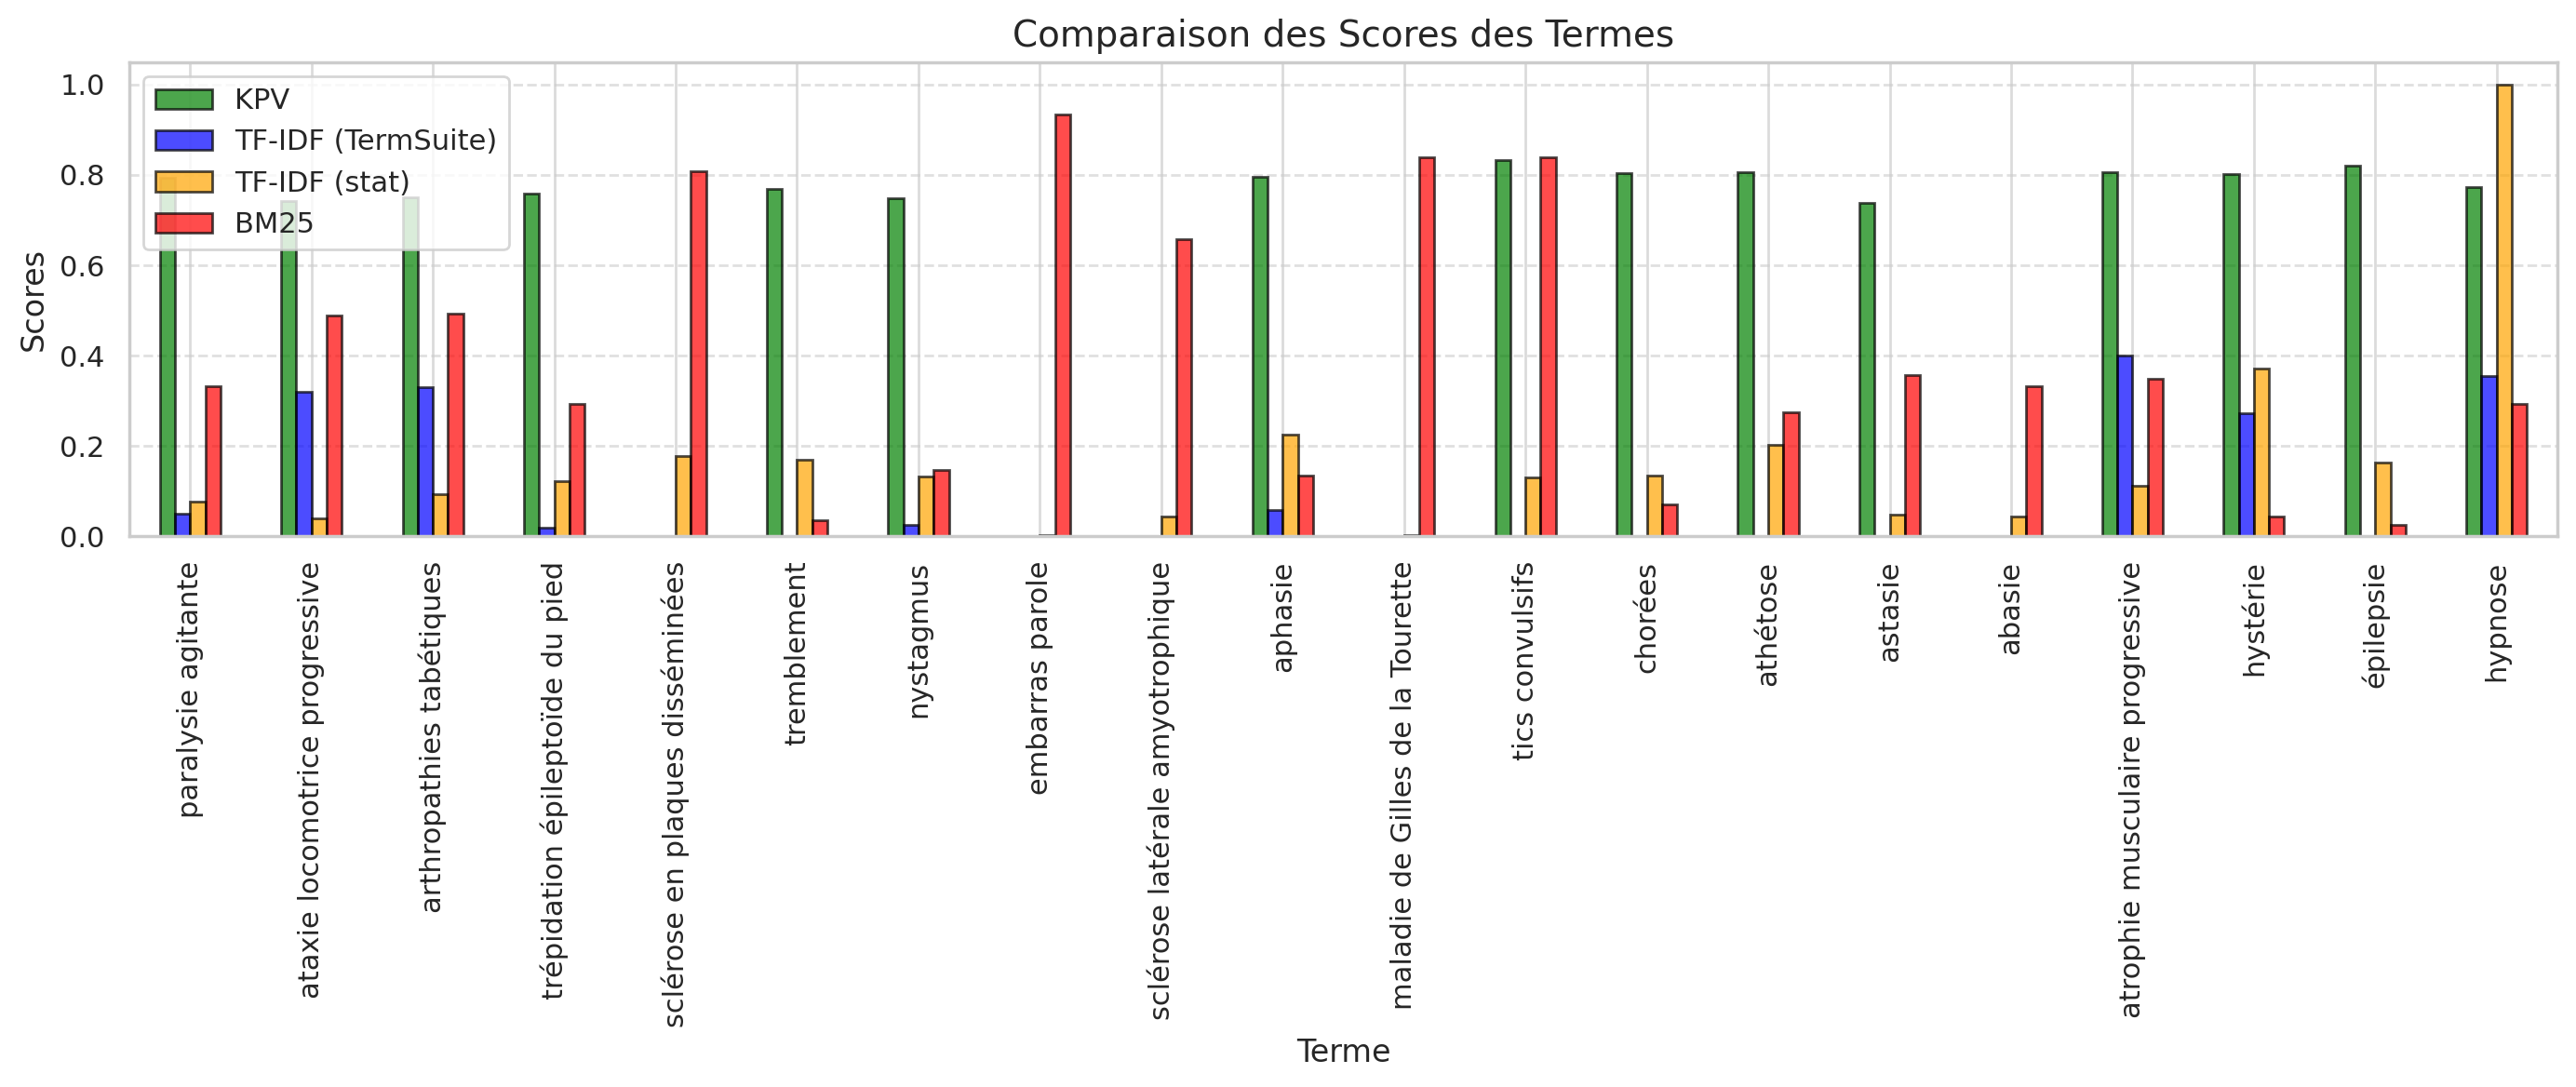
\includegraphics[width=\linewidth]{pic/termes_viz.png}
	\caption{Visualisation des scores de pertinences pour chaque terme de référence}
	\label{fig:ling_out_TAL}
\end{figure}
\end{frame}

%\begin{frame}{\textit{PatternRank}}
%	Les termes les plus pertinents dans \og{}Autres\fg{} :
%\begin{table}[h]
%	\centering
%	\begin{tabular}{|l|l|c|}
%		\hline
%		\textbf{Terme} & \textbf{Synonyme} & \textbf{Score} \\
%		\hline
%		\texttt{tics convulsifs} & \bolder{syndrome de Tourette} & \textsc{0.8331} \\
%		\texttt{état parkinsonien} & \bolder{maladie de Parkinson} & 0.7936 \\
%%		\texttt{paralytiques agitants} & \bolder{maladie de Parkinson} & 0.7851 \\
%		\hline
%	\end{tabular}
%\end{table}
%\end{frame}





\begin{frame}{Chronologie d'une locution : indice de croissance de l'impact ?}
\begin{figure}[h] % Use [H] to force the figure to stay in place
	\begin{itemize}
		\item évolution de la fréquence des termes au sein des deux corpus
		\item convergence entre des termes : fin \textsc{XIX}\ieme{}, début \textsc{XX}\ieme{} s.
		\begin{itemize}
				\item \textit{ppm} : nombre d’occurrences par million de mots 
		\end{itemize}
	\end{itemize}
	\centering
	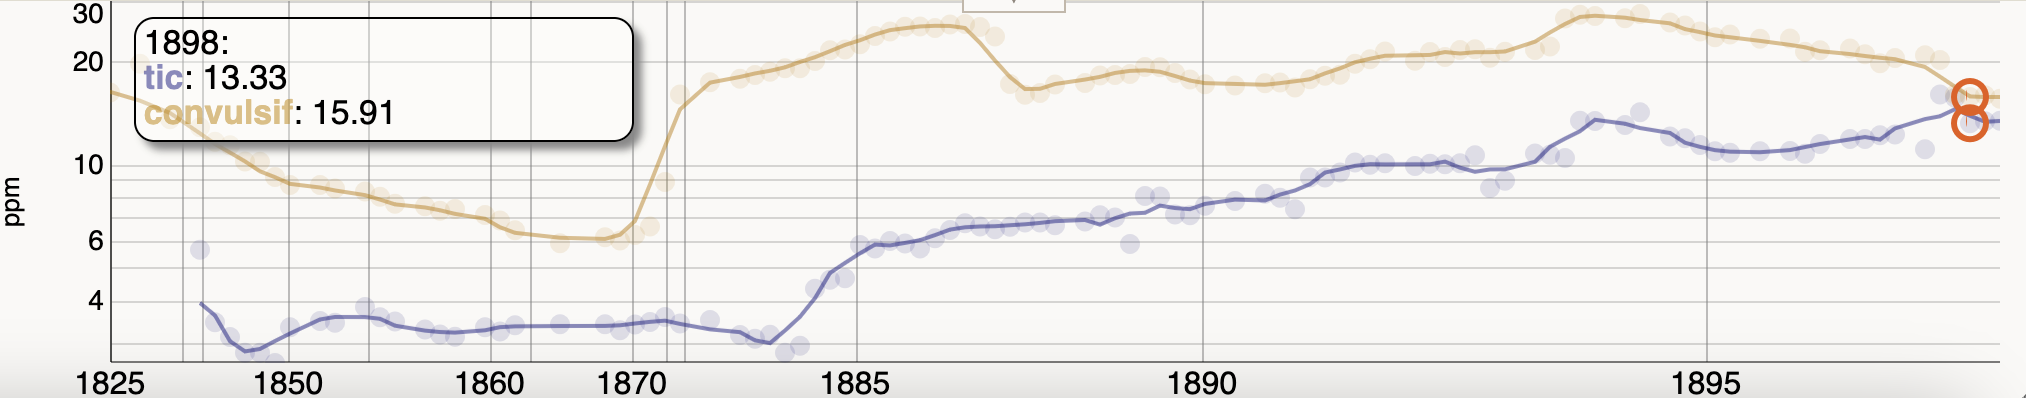
\includegraphics[width=\linewidth]{pic/tics_convulsifs.png}
	\caption{Chronologie de la fréquence du terme \textit{tic convulsif}.}
	\label{fig:ling_out_TAL}
\end{figure}

\begin{figure}[h]
	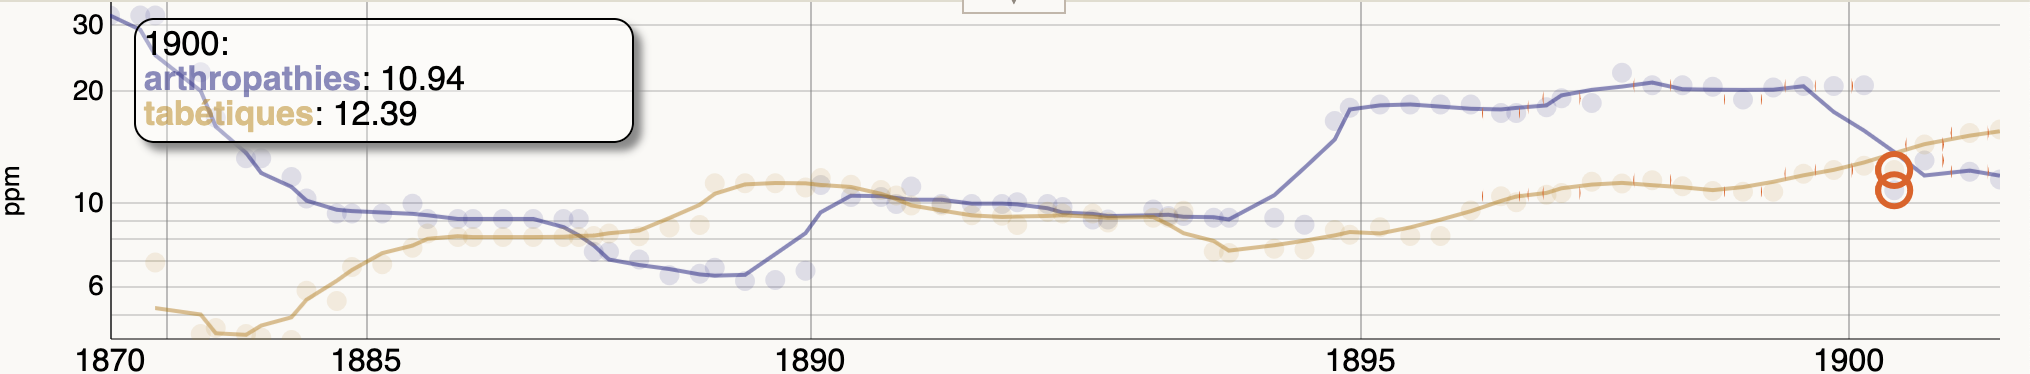
\includegraphics[width=\linewidth]{pic/arthropathies_tabetiques.png}
\caption{Chronologie de la fréquence du terme \textit{arthropathies tabétiques}.}
\label{fig:ling_out_TAL}
\end{figure}
\end{frame}

\section[Conclusion]{Conclusion}
\begin{frame}{Conclusion}
	\begin{enumerate}
		\item 	\textit{PatternRank} : la méthode la plus fiable par rapport aux autres méthodes ?
		\begin{itemize}
			\item capture la sémantique jusqu'aux pentagrammes
			\begin{itemize}
%				\item quadrigrammes : \textit{sclérose cérébrale tubéreuse hypertrophique} 
				\item \textit{méningite syphilitique hémorragique fibrineuse aiguë}
			\end{itemize}
			\item produit des scores de pertinence plus élevés
			\begin{itemize}
				\item exception : scores BM25 (\textit{SLA}, \textit{embarras parole}) et TF-IDF (\textit{hypnose})
			\end{itemize}
		\end{itemize}
		
		\item 	Les termes les plus impactants $\rightarrow$ syndrome de Tourette.
		
		\item Absence des scores pour les termes comme \textit{SEP} et SLA :
		\begin{itemize}                                        
			\item solution : chercher leurs symptomes ou leurs descriptions :
			\begin{itemize}
				\item  \textit{amyotrophie spinale progressive}, \textit{secousses nystagmiques}$\dots$
			\end{itemize}
		\end{itemize}
	\end{enumerate}
	

		
	\end{frame}
%
%\section[Approche supervisée]{Approche supervisée}
%\input{2_methodo}
%\input{supervise}
%\section[Approche non supervisée]{Approche non supervisée}
%%\begin{frame}{Extraction des phrases-clés}
%\og{}\textcolor{deepblue}{Phrases-clés}\fg{}, angl. \textit{keyphrases}
%\begin{itemize}
%\item séquences de plusieurs mots (ex. \textit{sclérose latérale amyotrophique})
%\item reflètent plus précisément le contexte sémantique du texte \\\small{$\neq$ mots-clés, angl. \textit{keywords} : unigrammes de mot (ex. \textit{sclérose})}
%\end{itemize}
%\bigskip
%%\centering
%%Extraction de \og{}phrases-clés\fg{} (angl. \textit{keyphrases})
%%\\~\\
%%\begin{block}{Extraction de phrases-clés}
%%\justifying
%%Processus de \underline{sélection} automatique d'un petit ensemble de phrases les plus pertinentes à partir d'un texte donné \citep{schopf2022}.
%%\end{block}
%%\begin{block}{Prédiction de phrases-clés}
%%\justifying
%%Processus de \underline{génération} des phrases-clés qui résument parfaitement un document donné \citep{xie2023}.
%\begin{columns}[t,onlytextwidth]
%\column{.45\textwidth}
%\textcolor{violet}{Extraction}
%\justifying
%
%Processus de \underline{sélection} automatique d'un petit ensemble de phrases les plus pertinentes à partir d'un texte donné.
%\vspace{-0.2cm}
%\begin{flushright}
%\small{\citep{schopf2022}}
%\end{flushright} 
%\column{.45\textwidth}
%\textcolor{violet}{Prédiction}
%\justifying
%
%Processus de \underline{génération} des phrases-clés qui résument parfaitement un document donné.
%\vspace{0.3cm}
%\begin{flushright}
%\small{\citep{xie2023}}
%\end{flushright}
%\end{columns}%Extraction de phrases-clés
%%
%%Processus de \underline{sélection} automatique d'un petit ensemble de phrases les plus pertinentes à partir d'un texte donné \citep{schopf2022}.
%%
%%\begin{block}{Prédiction de phrases-clés}
%%\justifying
%%Processus de \underline{génération} des phrases-clés qui résument parfaitement un document donné \citep{xie2023}.
%%\end{block} 
%\end{frame}

\begin{frame}{Extraction des phrases-clés : méthode \texttt{keybert}}
	\begin{enumerate}
		\small
		\item entrée : un document
		\item tokénisation du document en phrases-clés candidates (PCC)
		\item génération des plongements du doc. et des PCC par un modèle de langage
		\item calcul de la similarité cosinus entre le document et les PC
	\end{enumerate}
	\begin{figure}
		\centering
		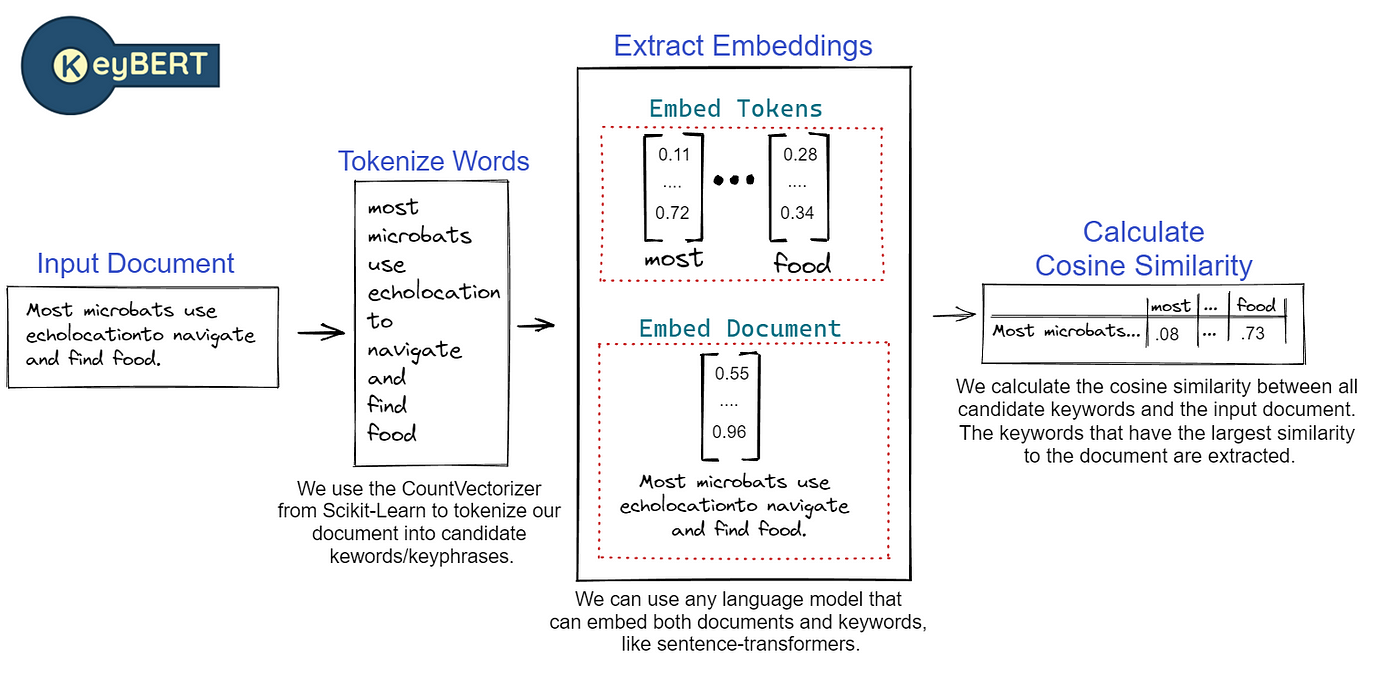
\includegraphics[width=80mm,scale=0.5]{pic/keybert.png}
		\caption{\textit{Pipeline} de la librairie \texttt{keybert} \citep{grootendorst2020keybert}.}
		\label{fig:enter-label}
	\end{figure}
\end{frame}

\begin{frame}{Extraction des phrases-clés : méthode \textit{PatternRank}\\
		\quad \quad \quad\ \quad \quad \quad \quad \quad \quad \quad \ \ \ \ \ \small{Librairie \texttt{keyphrase-vectorizers}}}
	%\begin{itemize}
	%\item extraction des phrases-clés non-supervisée
	%\item exploite des modèles de langues pré-entraînés + parties du discours
	%\end{itemize}
	\begin{enumerate}
		\small
		\item entrée : un seul document texte tokenisé
		\item étiquetage des tokens avec les balises du partie du discours (POS)
		\item sélection des tokens selon le motif POS $\rightarrow$ phrases-clés candidates (PCC)
		\item génération des plongements du doc. et des PCC par un modèle de langue
		\item calcul des similarités cosinus entre ces deux types de plongements +  \\classement des PCC par ordre décroissant
		\item extraction des \textit{N} PC les plus représentatives
	\end{enumerate}
	\begin{figure}
		\centering
		\includegraphics[width=110mm,scale=0.5]{pic/patternrank\_workflow.png}
		\caption{\textit{Workflow} de la méthode \textit{PatternRank} \citep{schopf2022}.}
		\label{fig:enter-label}
	\end{figure}
	\notecite{schopf2022}
\end{frame}



%\section[Conclusion]{Conclusion et recherches futures}
%\begin{frame}{Conclusion et perspectives}
	\begin{enumerate}
		\item 	\textit{PatternRank} : la méthode la plus robuste
		\begin{itemize}
			\item capture la sémantique jusqu'aux pentagrammes
			\begin{itemize}
				%				\item quadrigrammes : \textit{sclérose cérébrale tubéreuse hypertrophique} 
				\item \textit{méningite syphilitique hémorragique fibrineuse aiguë}
			\end{itemize}
			\item produit des scores de pertinence plus élevés
			\begin{itemize}
				\item exception : scores BM25 (\textit{SLA}, \textit{embarras parole}) et TF-IDF (\textit{hypnose})
			\end{itemize}
		\end{itemize}
		
		\item 	les termes les plus impactants dans les corpus :
		\begin{itemize}
			\item Charcot : \textit{hystérie}, \textit{astasie-abasie}, \textit{embarras parole}
			\item Autres :  \textit{hypnose}*, \textit{syndrome de Tourette}, \textit{arthropathies tabétiques}
		\end{itemize}

		%		\item Absence des scores pour les termes comme \textit{SEP} et SLA :
		%		\begin{itemize}                                        
			%			\item solution : chercher leurs symptomes ou leurs descriptions :
			%			\begin{itemize}
				%				\item  \textit{amyotrophie spinale progressive}, \textit{secousses nystagmiques}$\dots$
				%			\end{itemize}
			%		\end{itemize}
	\end{enumerate}
	
	\begin{alertblock}{\vspace*{-0.6mm}}
		\centering
		Les résultats sont alignés avec les faits historiques.
	\end{alertblock}
	
	\bigskip
	Recherches futures : tester les \textit{LLM} ou les \textit{LCM} (angl. \textit{Large Concept Models}) ?
\end{frame}
%\section[État de l'art]{État de l'art}
%\input{sota}
%\section[\textit{PatternRank}]{\textit{PatternRank}}
%\input{patternrank}



% \appendix

\begin{frame}[allowframebreaks]{Références}
\printbibliography

\end{frame}

\end{document}